\documentclass[aspectratio=169]{beamer}

% ---------- Theme ----------
\usetheme{Madrid}
\usecolortheme{default}

% ---------- Packages ----------
\usepackage[utf8]{inputenc}
\usepackage{graphicx}
\usepackage{amsmath}
\usepackage{booktabs}
\usepackage[table]{xcolor}
\definecolor{skyblue}{HTML}{CEDAEB}
\graphicspath{{images/}}
\usepackage{tikz}
\usepackage{times}
\usepackage{helvet}
\usepackage{courier}
\usefonttheme{serif}
\setlength{\abovedisplayskip}{4pt}
\setlength{\belowdisplayskip}{4pt}
\setlength{\abovedisplayshortskip}{2pt}
\setlength{\belowdisplayshortskip}{2pt}

\setbeamertemplate{navigation symbols}{} %% remove symbols navigations
\setbeamerfont{normal text}{size=\small}


% ---------- Title Info ----------
\title[Efficient BCD with RALA]{Efficient Multi-Temporal Building Change Detection\\
with Reduced-Rank Linear Attention}
\author[R. Acuña]{Ricardo Amiel Acuña Villogas}
\institute[UTEC - Ginia]{
UTEC - Ginia: Urban Data Analysis\\
Advisor: Rensso Victor Hugo Mora Colque \\
Co-Advisors: Germain García-Zanabria, Cristian José López del Álamo
}
\date{March 9, 2026}

% ---------- Begin ----------
\begin{document}

% ---------- Title ----------
\begin{frame}
  \titlepage
\end{frame}

% ---------- Outline ----------
\begin{frame}{Content}
\tableofcontents
\end{frame}

% =========================================================
\section{Introduction}

\begin{frame}{Building Change Detection}

\begin{columns}[T]
% ---------- Left column ----------
\begin{column}{0.42\textwidth}

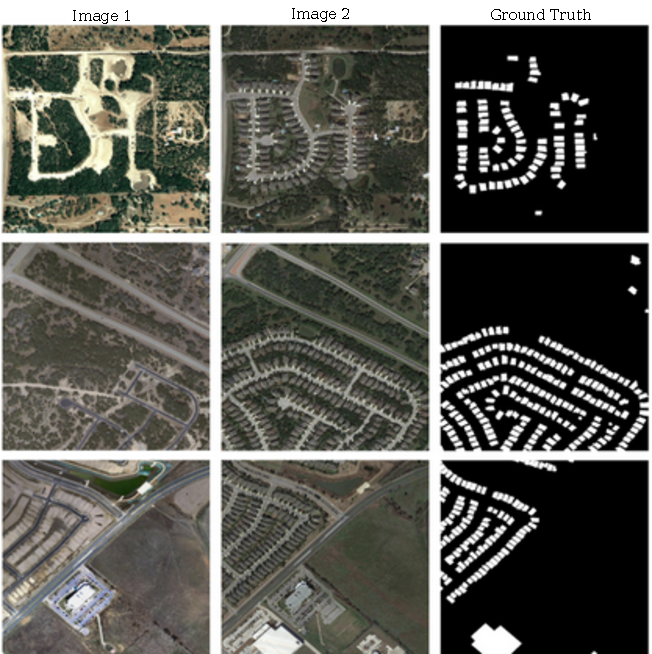
\includegraphics[
  width=\linewidth,
  height=0.7\textheight,
  keepaspectratio
]{vectorized-LEVIRCD.pdf}

\end{column}

% ---------- Right column ----------
\begin{column}{0.48\textwidth}

\small
\textbf{Building Change Detection (BCD)} compares \textbf{bi-temporal satellite images} to identify construction, demolition, or structural change.

\vspace{0.4cm}

\textbf{Why it matters}
\begin{itemize}
    \item Urban growth monitoring.
    \item Disaster response.
    \item Security and regulation.
    \item Planning and poverty analysis.
\end{itemize}

\end{column}
\end{columns}

\vspace{0.3cm}
\footnotesize
\tiny{Reference: \textit{A Spatial-Temporal Attention-Based Method and a New Dataset for Remote Sensing Image Change Detection. (Zheng et al.)}}

\end{frame}



\begin{frame}{Motivation}

\begin{columns}[T]

% ---------- Left column ----------
\begin{column}{0.48\textwidth}
\centering

\begin{minipage}{\linewidth}
\centering
\includegraphics[
  height=0.6\textheight,
  keepaspectratio
]{PeruSAT.png}

\vspace{0.2cm}
\footnotesize
\tiny{Reference: Conida PeruSat-1 sample}
\end{minipage}

\end{column}

% ---------- Right column ----------
\begin{column}{0.48\textwidth}
\centering

\begin{minipage}{\linewidth}
\centering
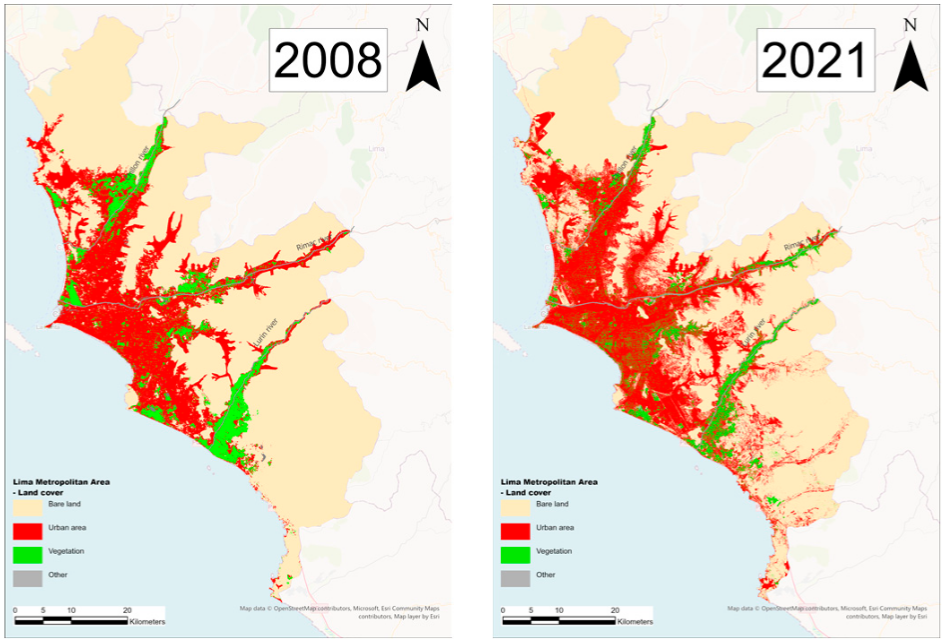
\includegraphics[
  height=0.6\textheight,
  keepaspectratio
]{LandCover.png}

\vspace{0.2cm}
\footnotesize
\tiny{Reference: Land cover changes in Lima Metropolitan Area for the years 2008 and 2021}
\end{minipage}

\end{column}

\end{columns}

\end{frame}



\begin{frame}{Challenges}

\begin{columns}[T]

% ---------- Left column ----------
\begin{column}{0.62\textwidth}
\centering

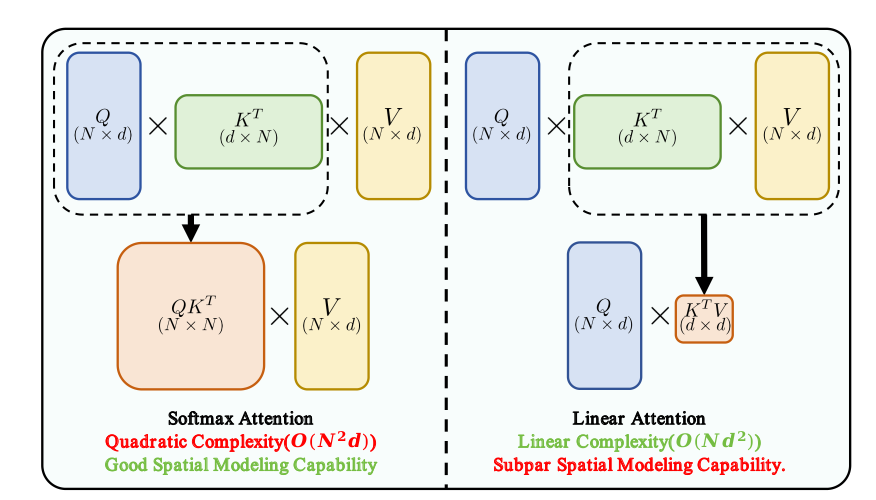
\includegraphics[
  height=0.6\textheight,
  keepaspectratio
]{Attention.png}

\end{column}

% ---------- Right column ----------
\begin{column}{0.34\textwidth}

\small
\begin{itemize}
    \item High computational cost: $\mathcal{O}(N^2)$.
    \item Large memory footprint.
    \item Small feasible batch sizes.
    \item Bi-temporal processing doubles computation.
    \item Limits deployment on large or OOD datasets.
\end{itemize}

\end{column}

\end{columns}

\vspace{0.25cm}

% ---------- Reference (aligned with left image) ----------
\hspace*{0.04\textwidth}
\parbox{0.62\textwidth}{
\footnotesize
\tiny{\textit{Reference: Breaking the Low-Rank Dilemma via Linear Attention} (Fan et al.)
}}

\end{frame}



\begin{frame}{Main Goal}

\begin{center}
{\Large\bfseries
Design a computationally efficient attention mechanism that reduces cost while preserving segmentation accuracy.
}
\end{center}

\end{frame}



\begin{frame}{Goals}
\begin{itemize}
    \item Reduce VRAM usage and FLOPs in the encoder.
    \item Increase feasible batch sizes for large-scale BCD training.
    \item Maintain comparable performance on LEVIR-CD and DSIFN-CD.
    \item \textbf{Scope}:  Train and validation on public benchmarks LEVIR-CD  (Zheng et al.) and DSIFN-CD (Shen et al.).
\end{itemize}
\end{frame}



% =========================================================
\section{Approach}

\begin{frame}{State of the Art in BCD}

\begin{center}
\begin{minipage}{0.95\linewidth}
\centering

\begin{tikzpicture}
\node[anchor=south west, inner sep=0] (img) at (0,0)
{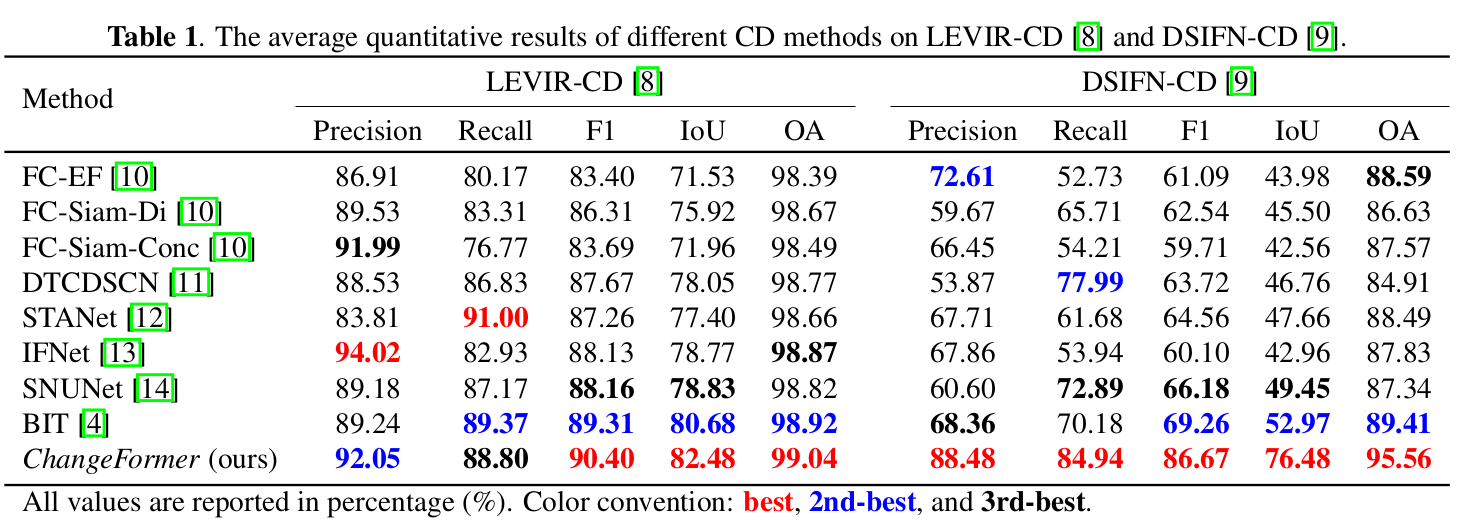
\includegraphics[
  width=\linewidth,
  height=0.65\textheight,
  keepaspectratio
]{SOTA.png}};

% ---- Dashed rectangle (HIGHLIGHT) ----
\draw[
  dashed,
  line width=1pt,
  rounded corners=4pt,
  blue
]
(0.1,0.45) rectangle (14.3,1.5);
\end{tikzpicture}

\vspace{0.2cm}
\footnotesize
\tiny{\textit{Reference: A Transformer-based Siamese Network for Change Detection} (Bandara et al.)}

\end{minipage}
\end{center}

\end{frame}



\begin{frame}{Baseline: ChangeFormer}

\begin{center}
\begin{minipage}{0.95\linewidth}
\centering

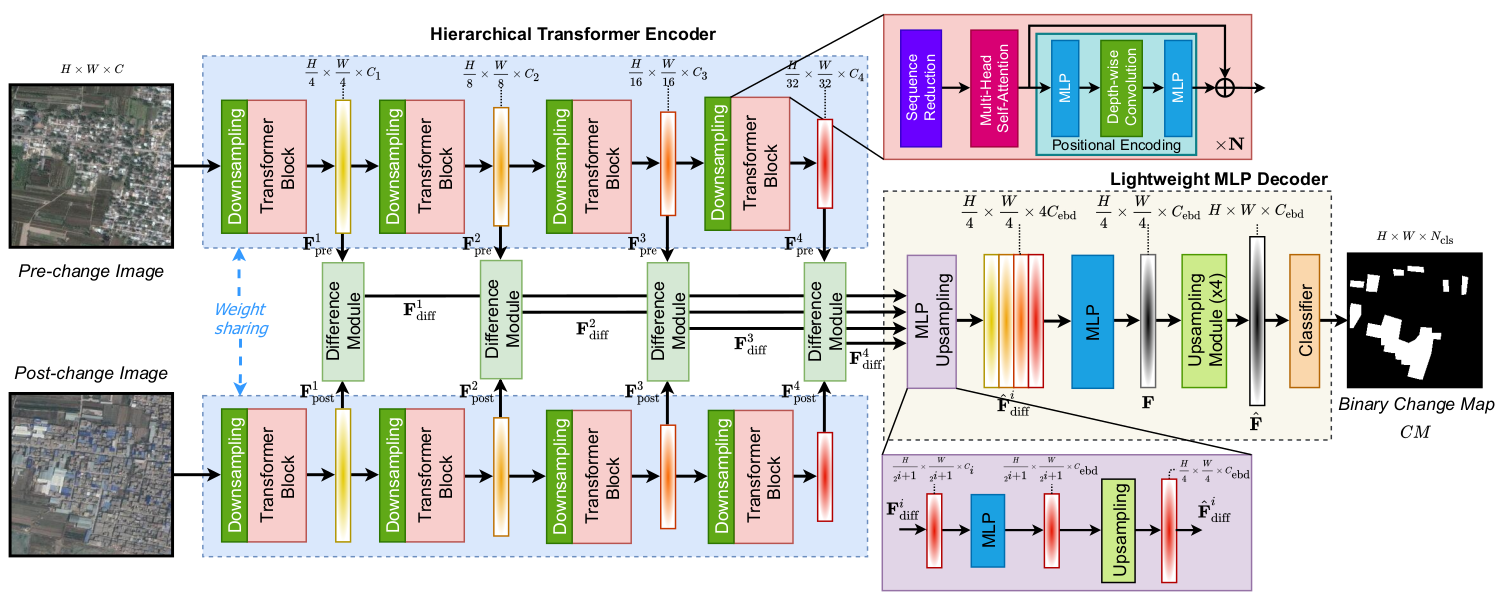
\includegraphics[
  width=\linewidth,
  height=0.65\textheight,
  keepaspectratio
]{ChangeFormer.png}

\vspace{0.2cm}
%\footnotesize
\tiny{\textit{Reference: A Transformer-based Siamese Network for Change Detection} (Bandara et al.)}

\end{minipage}
\end{center}

\end{frame}



\begin{frame}{Rank-Augmented Linear Attention (RALA)}

\begin{columns}[T]

% ---------- LEFT COLUMN: Image + Reference ----------
\begin{column}{0.45\textwidth}

\begin{center}
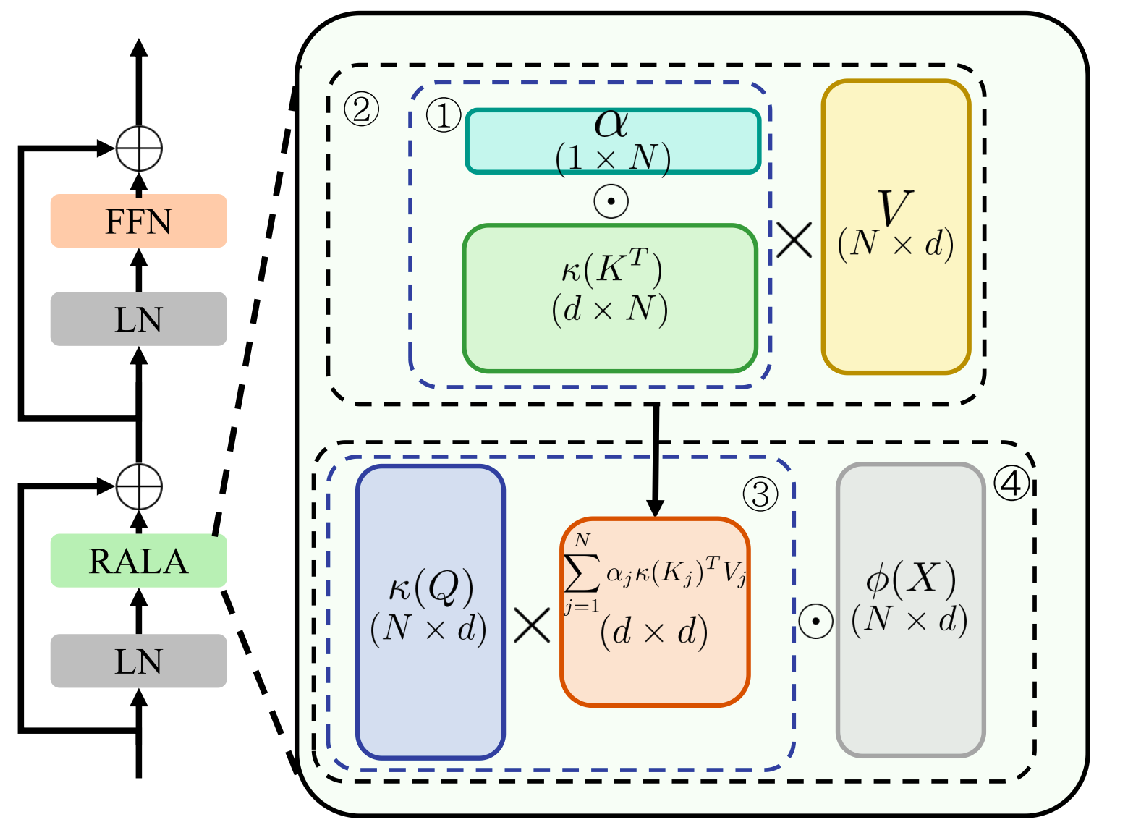
\includegraphics[
  width=\linewidth,
  height=0.6\textheight,
  keepaspectratio
]{RALA.png}
\end{center}

\vspace{0.8cm}
\footnotesize
\tiny{\textit{Reference: Breaking the Low-Rank Dilemma via Linear Attention} (Fan et al.)}

\end{column}

% ---------- RIGHT COLUMN: Mathematics ----------
\begin{column}{0.55\textwidth}

\footnotesize

\textbf{Linear Attention}
\[
\mathrm{Attn}_{\text{lin}}(Q,K,V)
= \kappa(Q)\big(\kappa(K)^\top V\big)
\]

\textbf{Global Query}
\[
Q_g = \frac{1}{N}\sum_{i=1}^{N} Q_i
\]

\textbf{Token Weights}
\[
\alpha_j
= N \cdot
\frac{\exp\!\big(Q_g \kappa(K_j)^\top\big)}
{\sum_{m=1}^{N}\exp\!\big(Q_g \kappa(K_m)^\top\big)},
\qquad
\sum_{j=1}^{N} \alpha_j = N
\]

\textbf{Key–Value Aggregation Buffer}
\[
B = \sum_{j=1}^{N} \alpha_j\, \kappa(K_j)^\top V_j
\]

\textbf{Modulated Output}\;
$Y_i = \phi(X_i) \odot \big(\kappa(Q_i)\, B\big)$

\end{column}

\end{columns}

\end{frame}




\begin{frame}{Datasets: LEVIR-CD}

\begin{center}
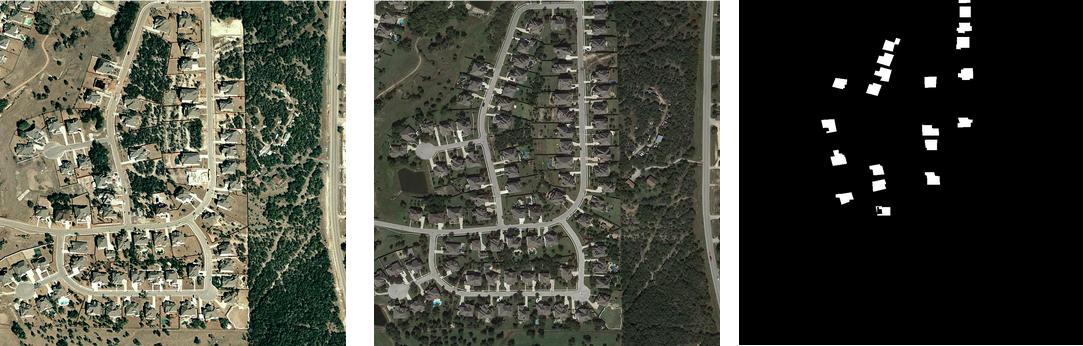
\includegraphics[
  width=0.95\linewidth,
  height=0.7\textheight,
  keepaspectratio
]{LEVIR2.png}
\end{center}

\vspace{0.3cm}

\vspace{0.2cm}
\footnotesize
\tiny{\textit{Reference: A Spatial-Temporal Attention-Based Method and a New Dataset for Remote Sensing Image Change Detection} (Zheng et al.)}

\end{frame}


\begin{frame}{Datasets: DSIFN-CD}

\begin{center}
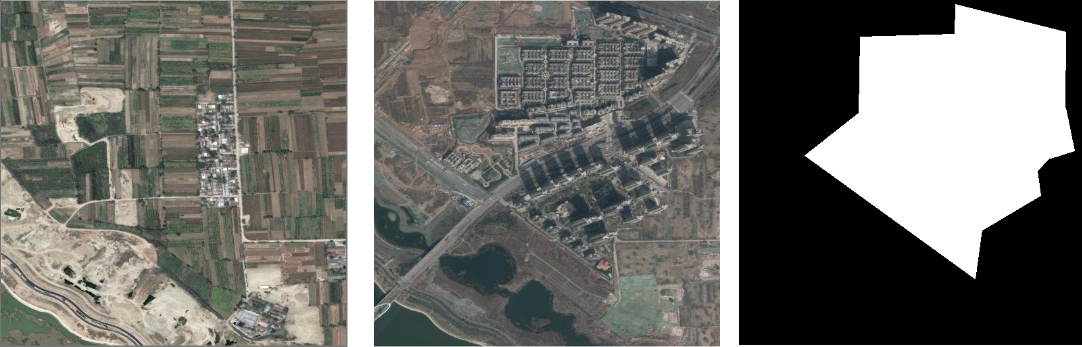
\includegraphics[
  width=0.95\linewidth,
  height=0.7\textheight,
  keepaspectratio
]{DSIFN2.png}
\end{center}

\vspace{0.3cm}

\vspace{0.2cm}
\footnotesize
\tiny{\textit{Reference: A Dense Siamese Network for Change Detection in Remote Sensing Images} (Shen et al.)}

\end{frame}


% =========================================================
\section{Discussion}

\begin{frame}{Segmentation Accuracy}

\centering
\footnotesize

\resizebox{0.95\linewidth}{!}{
\begin{tabular}{lcccc}
\hline
\textbf{Model} & \textbf{Dataset} & \textbf{F1} & \textbf{IoU} & \textbf{OA} \\
\hline
SNUNet-CD      & LEVIR-CD & 88.16 & 78.83 & 98.82 \\
BIT            & LEVIR-CD & 89.31 & 80.68 & 98.92 \\
ChangeFormer   & LEVIR-CD & 90.40 & 82.48 & 99.04 \\
\rowcolor{skyblue}
RALA-CF (ours) & LEVIR-CD & \textbf{89.87} & \textbf{81.60} & \textbf{98.99} \\
\hline
SNUNet-CD      & DSIFN-CD & 66.18 & 49.45 & 87.34 \\
BIT            & DSIFN-CD & 69.26 & 52.97 & 89.41 \\
ChangeFormer   & DSIFN-CD & 86.67 & 76.48 & 95.56 \\
\rowcolor{skyblue}
RALA-CF (ours) & DSIFN-CD & \textbf{84.07} & \textbf{73.96} & \textbf{92.44} \\
\hline
\end{tabular}
}

\vspace{0.2cm}
\tiny{\textit{Reference: Efficient Multi-Temporal Building Change Detection with Reduced-Rank Linear Attention} (Acuña et al.)}

\end{frame}




\begin{frame}{Efficiency Results}

\centering
\footnotesize

\resizebox{0.9\linewidth}{!}{
\begin{tabular}{lccc}
\hline
\textbf{Model} & \textbf{Params (M)} & \textbf{GFLOPs} & \textbf{Peak VRAM (GB)} \\
\hline
ChangeFormer   & 247 & 248.77 & 27 \\
\rowcolor{skyblue}
RALA-CF (ours) & \textbf{243} & \textbf{228.62} & \textbf{21} \\
\hline
\end{tabular}
}

\vspace{0.25cm}
\tiny{\textit{Reference: Efficient Multi-Temporal Building Change Detection with Reduced-Rank Linear Attention} (Acuña et al.)}

\end{frame}



\begin{frame}{Efficiency Results (Batch Size)}

\centering
\footnotesize

\resizebox{0.95\linewidth}{!}{
\begin{tabular}{lcccc}
\hline
\textbf{Resolution} & \textbf{Model} & \textbf{Max Batch} & \textbf{VRAM at OOM (GB)} \\
\hline
\multirow{2}{*}{256$\times$256}
& ChangeFormer & 32 & 34 \\
& \rowcolor{skyblue} RALA-CF (ours) & \textbf{48} & \textbf{34} \\
\hline
\multirow{2}{*}{512$\times$512}
& ChangeFormer & 8 & 34 \\
& \rowcolor{skyblue} RALA-CF (ours) & \textbf{12} & \textbf{34} \\
\hline
\multirow{2}{*}{1024$\times$1024}
& ChangeFormer & 2 & 36 \\
& \rowcolor{skyblue} RALA-CF (ours) & \textbf{3} & \textbf{36} \\
\hline
\end{tabular}
}

\vspace{0.25cm}
\tiny{\textit{Reference: Efficient Multi-Temporal Building Change Detection with Reduced-Rank Linear Attention} (Acuña et al.)}

\end{frame}



\begin{frame}{Efficiency Results (Ablation Study)}

\centering
\footnotesize

\resizebox{0.7\linewidth}{!}{
\begin{tabular}{lcc}
\hline
\textbf{Variant} & \textbf{GFLOPs} & \textbf{VRAM (GB)} \\
\hline
Baseline MHSA & 86.17 & 12 \\
\rowcolor{skyblue}
Encoder: RALA (ours) & \textbf{76.95} & \textbf{8} \\
\hline
\end{tabular}
}

\vspace{0.25cm}
\tiny{\textit{Reference: Efficient Multi-Temporal Building Change Detection with Reduced-Rank Linear Attention} (Acuña et al.)}

\end{frame}




\begin{frame}{Attention Maps}

\begin{center}
\begin{tikzpicture}
\node[anchor=south west, inner sep=0] (img) at (0,0)
{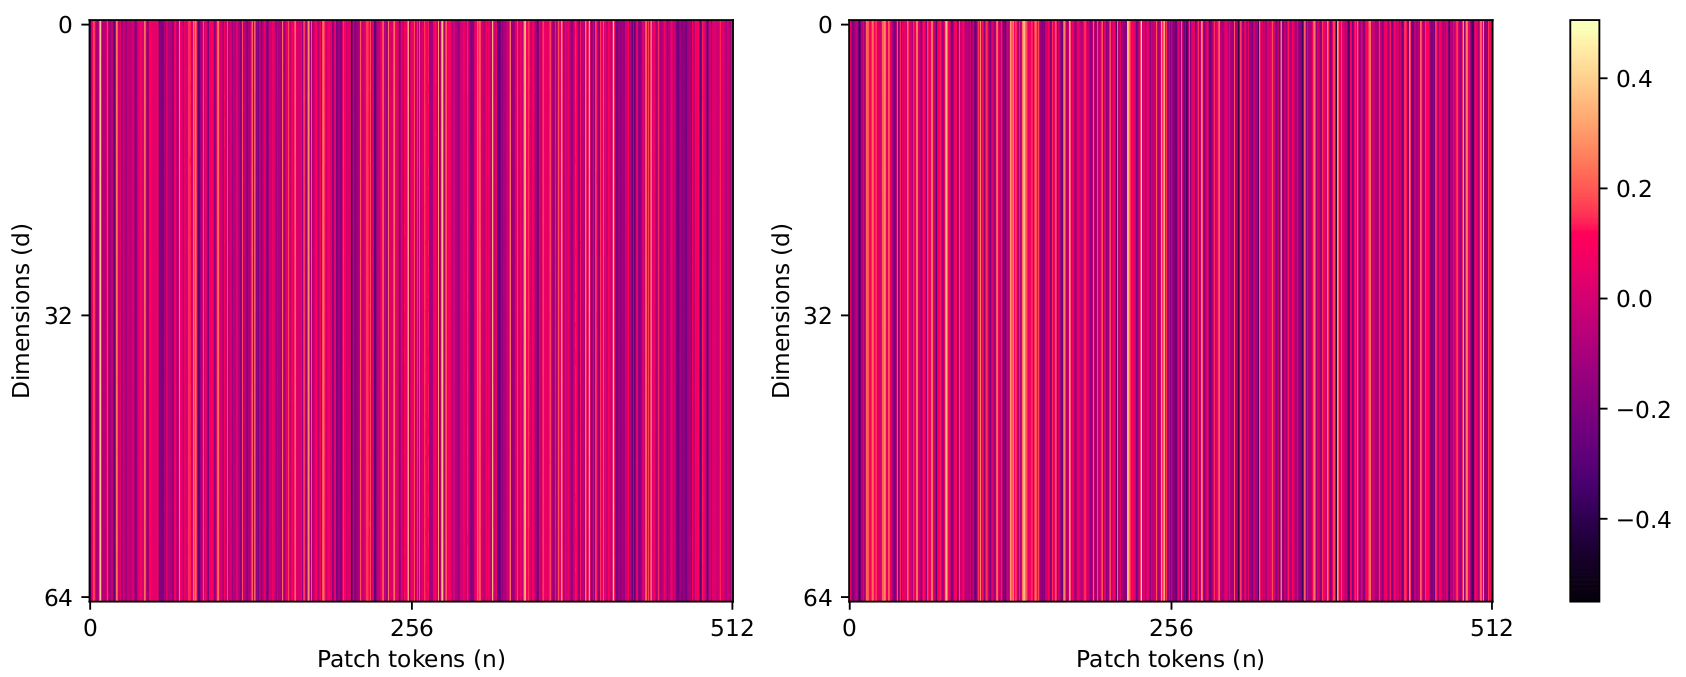
\includegraphics[
  width=0.95\linewidth,
  height=0.7\textheight,
  keepaspectratio
]{Attention-Maps2.png}};

% ---- Highlight rectangle (MHSA) ----
\draw[
  dashed,
  line width=1pt,
  rounded corners=3pt,
  yellow
]
(5.3,0.7) rectangle (6.0,5.6);

% ---- Highlight rectangle (RALA) ----
\draw[
  dashed,
  line width=1pt,
  rounded corners=3pt,
  yellow
]
(11.8,0.7) rectangle (12.5,5.6);
\end{tikzpicture}
\end{center}

\footnotesize
The highlighted regions illustrate subtle local differences in attention intensity; however, these minimal variations do not affect the global structure of attention. (Order: MHSA vs RALA)

\vspace{0.1cm}
\tiny{\textit{Qualitative comparison only. Colors denote normalized attention intensity.  
Reference: Acuña et al., Efficient BCD with RALA}}

\end{frame}




% =========================================================
\section{Limitations}

\begin{frame}{Limitations}
\begin{itemize}
    \item Encoder-only modification limits the magnitude of end-to-end speedups
    \item Efficiency gains increase with higher token counts, improvements are smaller at 256×256
    \item No enhancement to non-attention components
    \item Accuracy remains ultimately constrained by ChangeFormer’s original architecture
\end{itemize}
\end{frame}

% =========================================================
\section{Conclusions}

\begin{frame}{Conclusions}
\begin{itemize}
    \item Achieves \textbf{accuracy comparable} to ChangeFormer across benchmarks
    \item Avoids \textbf{low-rank collapse}, preserving stable attention patterns
    \item Reduces \textbf{attention-related FLOPs} and \textbf{peak VRAM consumption}
    \item Enables \textbf{larger batch sizes} and higher-resolution training under fixed GPU limits
    \item Provides a \textbf{strong accuracy–efficiency trade-off} for VHR building change detection
\end{itemize}
\end{frame}

% =========================================================
\section{Future Work}

\begin{frame}{Future Work}
\begin{itemize}
    \item Explore \textbf{more expressive kernel feature maps} for linear attention
    \item Integrate RALA into \textbf{multi-scale} and \textbf{multi-task BCD frameworks}
    \item Extend memory-efficient attention to \textbf{generative BCD models}
    \item Validate scalability in \textbf{larger, more heterogeneous datasets}, including Peruvian satellite imagery (PeruSAT-1)
\end{itemize}
\end{frame}

% =========================================================
\section*{References}

\begin{frame}{References (1/3)}
\footnotesize
\begin{enumerate}
\item Bandara, W.G.C., \& Patel, V.M. (2022). \textit{ChangeFormer}. IGARSS.
\item Zheng, G. et al. (2020). \textit{LEVIR-CD}. Remote Sensing.
\item Shen, Y. et al. (2021). \textit{DSIFN-CD}. IEEE TIP.
\item Fang, J. \& Li, J. (2021). \textit{SNUNet-CD}. IEEE GRSL.
\item Chen, H. et al. (2022). \textit{BIT}. CVPR.
\item Zheng, X. et al. (2023). \textit{HFA-Net}. Pattern Recognition.
\item Teng, Y. et al. (2023). \textit{SwinCD}. Remote Sensing.
\item Vaswani, A. et al. (2017). \textit{Attention Is All You Need}. NeurIPS.
\item Dosovitskiy, A. et al. (2021). \textit{ViT}. ICLR.
\item Raghu, A. et al. (2023). \textit{Revenge of ViT}. LNCS.
\item Fan, Y. et al. (2024). \textit{ViTAR}. CVPR.
\item Fan, Q. et al. (2025). \textit{RALA}. ICLR.
\end{enumerate}
\end{frame}

\begin{frame}{References (2/3)}
\footnotesize
\begin{enumerate}
\setcounter{enumi}{12}
\item Daudt, R.C. et al. (2018). \textit{Fully Convolutional Siamese Networks}. ICIP.
\item Zhang, C. et al. (2020). \textit{Image Fusion Network}. ISPRS JPRS.
\item Hussain, M. et al. (2013). \textit{Change Detection Review}. ISPRS JPRS.
\item Zhang, C. et al. (2020). \textit{Survey on BCD}. ISPRS JPRS.
\item Shafique, A. et al. (2022). \textit{Deep Learning CD Review}. Remote Sensing.
\item Katharopoulos, A. et al. (2020). \textit{Transformers are RNNs}. ICML.
\item Choromanski, K. et al. (2021). \textit{Performer}. ICLR.
\item Wang, S. et al. (2020). \textit{Linformer}. NeurIPS.
\item Xiong, Y. et al. (2021). \textit{Nyströmformer}. AAAI.
\item Liu, Z. et al. (2021). \textit{Swin Transformer}. ICCV.
\item Wei, C. et al. (2023). \textit{Sparsifiner}. CVPR.
\item Yang, L. et al. (2021). \textit{Deep Siamese Networks for CD}. Remote Sensing.
\end{enumerate}
\end{frame}

\begin{frame}{References (3/3)}
\footnotesize
\begin{enumerate}
\setcounter{enumi}{24}
\item Zhao, S. et al. (2023). \textit{Dual Encoder–Decoder CD}. IEEE TGRS.
\item Tan, X. et al. (2024). \textit{Segment Change Model}. IGARSS.
\item Guo, H. et al. (2021). \textit{Building Footprint Update}. RSE.
\item Cao, Y. \& Huang, X. (2023). \textit{FFCTL}. RSE.
\item Xiao, W. et al. (2024). \textit{CSCL-Net}. IJAEOG.
\end{enumerate}
\end{frame}

\begin{frame}{}

\begin{columns}[T]

% ---------- Left column ----------
\begin{column}{0.5\textwidth}
\vspace{1cm}
\Large
\textbf{Thank you.}

\vspace{0.5cm}
\normalsize
Code available at:

\vspace{0.2cm}
\small \texttt{github.com/ricardoamiel/RALA-ChangeFormer}

\vspace{0.8cm}
\Large
Questions?
\end{column}

% ---------- Right column ----------
\begin{column}{0.50\textwidth}
\centering
\vspace{0.6cm}

\includegraphics[
  width=0.7\linewidth,
  keepaspectratio
]{QR.png}
\end{column}

\end{columns}

\end{frame}


\end{document}
